% This is samplepaper.tex, a sample chapter demonstrating the
% LLNCS macro package for Springer Computer Science proceedings;
% Version 2.20 of 2017/10/04
%
\documentclass[runningheads]{llncs}
%
\usepackage[utf8]{inputenc}
\usepackage{graphicx}
\usepackage[british]{babel}
\usepackage{amsmath}
\usepackage[linesnumbered]{algorithm2e}
\usepackage{algorithmic}


\hyphenation{per-tur-ba-tion ad-ver-sa-ri-al Com-pu-ter sev-er-al doc-u-ment-ed Image-Net}
%\usepackage[backend=biber]{biblatex}
%\usepackage[backend=biber,style=splncs04]{biblatex}  %backend=biber is 'better'  

% Used for displaying a sample figure. If possible, figure files should
% be included in EPS format.
%
% If you use the hyperref package, please uncomment the following line
% to display URLs in blue roman font according to Springer's eBook style:
% \renewcommand\UrlFont{\color{blue}\rmfamily}

% ---- Bibliography ----
%
% BibTeX users should specify bibliography style 'splncs04'.
% References will then be sorted and formatted in the correct style.
%
\DeclareMathOperator{\sgn}{sgn}


\newcommand{\xn}{\ensuremath{\mathbf{x_0}}}
\newcommand{\xb}{\ensuremath{\mathbf{x}}}
\newcommand{\rb}{\ensuremath{\mathbf{r}}}
\newcommand{\vb}{\ensuremath{\mathbf{v}}}
\newcommand{\kf}{\ensuremath{k_{\!f}}}
\newcommand{\kg}{\ensuremath{k_{\!g}}}
\bibliographystyle{splncs04}
\begin{document}
%
\title{Combining Universal Adversarial Perturbations}%\thanks{Supported by organization x.}
%
\titlerunning{Combining Universal Adversarial Perturbations}
% If the paper title is too long for the running head, you can set
% an abbreviated paper title here
%
\author{Maurus K\"uhne\inst{1}\orcidID{0000-0002-4205-3552} \and
Beat Tödtli\inst{2}\orcidID{0000-0003-3674-2340}} %\and
%Third Author\inst{3}\orcidID{2222--3333-4444-5555}}
%
\authorrunning{M. Kühne and B. Tödtli}
% First names are abbreviated in the running head.
% If there are more than two authors, 'et al.' is used.
%
\institute{Fernfachhochschule Schweiz\\
\email{maurus.kuehne@students.ffhs.ch}\and
Institut für Informations- und Prozessmanagement, FHS St. Gallen \\
\email{beat.toedtli@ost.ch}
}
%
\maketitle              % typeset the header of the contribution
%
\begin{abstract}
Universal adversarial perturbations (UAPs) are small perturbations imposed on images that are able to fool a single convolutional neural network image classifier. They have been shown to generalise well to other neural networks. Here, we report on our reproduction effort of the results given in a work by Moosavi-Dezfooli et al. on UAPs and study two methods to construct UAPs for several neural networks. While the results are not strong enough to make general conclusions, they suggest that UAPs indeed profit from being constructed on several neural networks. Also, we show that a linear interpolation between two UAPs does not produce a viable UAP on both networks.
%\cite{yu_generating_2018}
\keywords{Adversarial Training\and Universal Adversarial Perturbation}
\end{abstract}
%
%
%
\section{Introduction}
The discovery of Szegedy et al.~\cite{Szegedy_2014} that several machine learning models including deep neural networks are vulnerable to \emph{adversarial attacks} was seminal for a new subfield of studying deep learning. Probably the most intriguing, but also unsettling result was that adversarial examples can be made quite imperceptible to the human eye while still fooling a convolutional neural network to misclassify the image~\cite{goodfellow_2014}. Subsequent work has developed various algorithms in a variety of white-box, grey-box and black-box attack scenarios as well as defensive strategies such as adversarial training~\cite{REN2020346}. 
Moosavi-Dezfooli et al.~\cite{moosavidezfooli_universal_2017,moosavi-dezfooli_deepfool_2016} have demonstrated that \emph{universal} perturbations exist, i.e. that a single set of of pixel modifications can be found that fools a network on a large fraction of the training data set. Moreover, universal adversarial perturbations (UAPs) also fool other convolutional networks. The authors of~\cite{moosavidezfooli_universal_2017,moosavi-dezfooli_deepfool_2016} show good generalization results for UAPs generated with their procedure \emph{DeepFool}~\cite{moosavi-dezfooli_deepfool_2016} across different deep learning architectures.  

These results suggest that neural networks and convolutional neural networks for image classification in particular partly share a common structure that can be exploited by universal adversarial perturbations (UAPs) while yet other aspects are different. Thus, understanding UAPs provides a window into the weaknesses of neural networks. By building UAPs that are viable on several networks, a common weakness of those networks is identified. This in turn helps in building more robust networks, for example again by adversarial training. Even more generally, therefore, we view work on UAPs as one more way of (partly) approaching the bigger question of why neural networks with a large number of weights work at all (or when they don't).

In this context, we ask whether combining two neural networks in generating adversarial perturbations can improve the transferability of UAPs to new convolutional neural networks. We observe that in the approach by Moosavi-Dezfooli et al. \cite{moosavidezfooli_universal_2017,moosavi-dezfooli_deepfool_2016}, implementing such a combination is particularly simple. 
We report on our effort to reproduce their results, provide our code and investigate whether modifications of their UAP algorithm are able to improve the generalisation capability of UAPs. To do so, we devise modifications of the UAP generation algorithm that take into account several networks at the same time\footnote{Instead of combining UAPs from different networks, UAPs of networks trained on different data domains can be combined, as done e.g. by Naseer et al.~\cite{NIPS2019_9450}.}
Specifically, we assess whether incorporating information from a second neural network architecture improves the fooling rate of UAPs on a third neural network. We investigate three combination procedures and compare them with the original adversarial attack procedure.

Given the practical potential and relevance of Deep Learning and the potential security threats of adversarial perturbations, finding a robust resolution is important and urgent. However, research into the topic is hampered by the \emph{reproducibility crisis} in machine learning~\cite{raff2020quantifying}. Research results are often difficult to reproduce due to undocumented values for hyperparameters, software library versions etc.~\cite{Gundersen2018StateOT}. As this was also the case for our reproduction efforts of the UAP-results of Moosavi-Dezfooli et. al., we endorse the NeurIPS-2019 code submission policy by providing our code and including their reproducibility checklist.

%%Given the practical potential and relevance of Deep Learning and the potential security threats of adversarial perturbations, finding a robust resolution is important and urgent. However, research into the topic is hampered by the \emph{reproducibility crisis} in machine learning~\cite{raff2020quantifying}. A lot of research results, including on adversarial attacks, remain poorly documented in publications. While the methods described may be general enough to be useful for many similar applications, the published results are often difficult to reproduce due to undocumented values for hyperparameters, software library versions etc.~\cite{Gundersen2018StateOT}. Also, only in rare cases is it clear how well the published results generalise beyond the very specific data set that was used but not provided to produce the published results. While not being able to reproduce the generation of adversarial examples may seem beneficial at first sight, it is clear that a thorough resolution of such security issues requires a well-stated problem, including readily available state-of-the-art algorithms for the production of adversarial examples. They form the basis of being able to test deep learning systems against such attacks. As a step towards addressing these challenges, we endorse the NeurIPS-2019 code submission policy by providing our code and including their reproducibility checklist.

This paper is organised as follows. In Sec.~\ref{sec:relatedWork} we briefly review related work. In Sec.~\ref{sec:methods} we present the basic methods used to generate adversarial and universal adversarial perturbations as introduced by Moosavi-Dezfooli et al.~\cite{moosavidezfooli_universal_2017}. We then present three modifications of their UAP generation algorithm to combine UAPs for several networks. In Sec.~\ref{sec:Results} we first describe our reproduction effort of the original work of Moosavi-Dezfooli et al.~\cite{moosavidezfooli_universal_2017} to produce UAPs on a set of networks and provide our fooling rates. We then present our results on the three methods to produce UAPs for several networks and show that the transferability to a third network is improved. In Sec.~\ref{sec:Discussion} we discuss these results and conclude with Sec.~\ref{sec:conclusion}.

\section{Related Work}\label{sec:relatedWork}
Many authors have suggested adversarial perturbation generating methods in various different settings. These attempts often generate per-instance perturbations. Among the image-agnostic methods, i.e. those generating UAPs, there are both data-driven and data-independent techniques, white-box and black-box attacks (depending on whether the internal structure of the network to be attacked is accessible to the attacker) and whether the attack is targeted or not (i.e. whether a misclassification into a particular class is required, or whether any misclassification is counted as a success). For a review and references, see~\cite{Chaubey2020UniversalAP}. UAPs can be generated e.g. by gradient descent on a loss function or learned using generative models. These methods being data-driven, they require access to training data, preferably the training data of the network to be fooled. Data-independent techniques such as Fast Feature Fool~\cite{Mopuri2017FastFF} or GD-UAP~\cite{DBLP:journals/corr/abs-1801-08092} do not need this access, but usually have access to the internal state of the network to be fooled. Our approach is a data-dependent white-box attack closely tied to the UAPs of Moosavi-Dezfooli et al.~\cite{moosavidezfooli_universal_2017}.

Many of these methods generate perturbations that transfer well between different model architectures. As part of our contribution we seek methods that optimise the transferability of perturbations between models. Our approach tries to achieve this by using multiple models to generate perturbations.

\section{Methods}\label{sec:methods}
\subsection{General Setting}
Given an image classifier \(\hat{k}(\xb)=\sgn\left(f(\xb)\right)\) that is based on the sign of a classification function \(f:\mathbf{R}^n\rightarrow\mathbf{R}\), adversarial attacks seek a perturbation \(\vb\) such that \[\hat{k}(\xb+\vb)=\sgn\left(f(\xb+\vb)\right)\neq \sgn\left(f(\xb)\right)=\hat{k}(\xb).\] 
In the following we briefly describe the adversarial perturbation generating method DeepFool and its generalisations to UAPs in the multi-class classification setting. We then describe the two approaches analysed here to build UAPs from several networks.

\subsection{DeepFool}\label{sec:DeepFool}

In the generation procedure DeepFool~\cite{moosavi-dezfooli_deepfool_2016}, the perturbation \(\mathbf{v}\) for an image \(\xb\) is defined to be the shortest vector\footnote{In practice and also in our code, the vectors (elements of a vector space) such as \(\xb\) and \(\vb\) have additional structure such as (for images) height, width and depth that is used to implement the classifier \(\hat{k}\). In the field of Deep Learning these data structures are therefore often called \emph{tensors}.}
(using the \(L_p\)-norm \(\left\|.\right\|_p\)) such that \(\xb+\mathbf{v}\) lies on a decision boundary. 
If $f(\xb)$ is a linear function $f(\xb)=\mathbf{w} \xb+\mathbf{b}$, then \(\mathbf{v}\) can be shown to be \(\mathbf{v}=-\frac{f(\xb)}{\left\|\mathbf{w}\right\|_p^2}\mathbf{w}\). As \(f\) is nonlinear in general, the Taylor approximation of the function $f$ around \(\mathbf{x}\), \(f(\mathbf{x}+\mathbf{v})=f(\mathbf{x})+\left(\nabla f(\mathbf{x})\right)^T\mathbf{v}\) is used to iteratively reach the decision boundary. 
In the multi-class setting considered here, an additional step is required that identifies the closest decision boundary. 

\subsection{Universal Adversarial Perturbations with DeepFool}

Perturbations for each image in a dataset \(X\) (such as those generated using DeepFool) can be combined to form universal adversarial perturbations for a single network~\cite{moosavidezfooli_universal_2017}. The procedure is given in Alg.~\ref{alg:1a} for a classifier set $K$ with one element. Essentially, DeepFool perturbations of images that are not yet misclassified are added to obtain a universal perturbation. 
Whenever the norm of the perturbation becomes large, a rescaling is applied. The perturbation is scaled back to satisfy a norm bound given by \(\left\|\mathbf{v}\right\|_p\leq\xi\) (that potentially undoes the successful perturbation of some images). For a small value of \(\xi\), this ensures that the perturbation remains largely invisible.

Intriguingly, although the directions to the class boundaries vary for different training images, the resulting average over all image perturbations works well according to~\cite{moosavidezfooli_universal_2017}, even for other convolutional neural networks whose class boundaries might be expected to look rather different. 

\subsection{Multi-Classifier Universal Adversarial Perturbations}\label{sec:MultUAP}

In the following subsections, we detail two approaches to generating UAPs for several classifiers.

\subsubsection{Alternated Generation of Perturbations}
Since UAPs are constructed by adding up the perturbations generated using DeepFool, there is a natural way to combine perturbations generated by the two networks: We add up the contributions from all networks. We note that adding up the perturbations is not a commutative operation, since projections take place once the size (norm) of the perturbation becomes too large. The precise procedure used here is given in Alg.~\ref{alg:1a}. 

Variants of Alg.~\ref{alg:1a} exist that sample the images differently. One might for example generate perturbation by alternating the classifier for each image. We show this variant in Alg.~\ref{alg:1b}. We evaluate both variants and compare their performance in Tab.~\ref{tab:vergleich_comb}. 
 
\subsubsection{Interpolation Between UAPs on Individual Networks}
A simple yet instructive alternative to the above rather involved perturbation construction is given by a simple weighted average of the perturbation vectors generated on the individual networks. If we restrict our attention to the combination of two neural networks for now, then the weighted averages of the perturbations lie on a line in the high-dimensional vector space of images. In the following, we specifically investigate whether any perturbation lying on this line improves on the fooling capability of the two endpoints with respect to a third network.
More formally, given UAPs \(\mathbf{v}_f\) and \(\mathbf{v}_g\) of two neural networks $f$ and $g$, we consider \begin{equation}\label{eq:interp}
\mathbf{v}_{fg}\left(\lambda\right)=\lambda\,\mathbf{v}_f+\left(1-\lambda\right)\mathbf{v}_g
\end{equation}	
for values \(\lambda\in\left[0,1\right]\). We seek the value of $\lambda$ that maximises the average fooling rate over $f$, $g$ and a third network, given the current training data set.


\subsubsection{Outlook to Other Approaches}
We have also investigated other, more involved approaches that led to unsatisfactory results. In particular, we were interested in constructing a multi-class DeepFool procedure that uses the gradients of two networks towards the next class boundary to compute a perturbation of a single image. One might try to find perturbations towards class boundaries that are aligned as much as possible, but where the class boundaries correspond to different classes in different networks. As of now, these attempts have not provided efficient UAPs for multiple networks.

\begin{figure}
\begin{algorithm}[H]
\SetAlgoLined
{\bf Input}:Data set \(X\), set of classifiers \(K\), desired norm \(\left\|.\right\|_p\) of
the perturbation \(\xi\)\\
{\bf Output}: Universal perturbation vector \(\vb\)\\
Initialise \(\vb \gets 0\)\\
\While{\textup {Average fooling rate is too low and max. number of iterations is not reached}}{
\ForEach{\(\mathrm{image~}\xb\in X\)  }{ 
\ForEach{\(\hat{k}\in K\)  }{ 
	\If{ \(\hat{k}(\xb)=\hat{k}(\xb+\vb)\)}{
		\(\Delta \vb\gets\texttt{DeepFool} (\xb+\vb,\hat{k})\)\\
	\(\vb\gets \vb+\Delta \vb\)  \\
	\(\vb\gets \sqrt{\xi}\vb/\left\|\vb\right\|_p\)
}  }
} 
Shuffle \(X\)
 }
\Return \vb
 \caption{Computation of universal adversarial perturbations for multiple neural networks. The function \texttt{DeepFool} computes an adversarial perturbation as described in Sec.~\ref{sec:DeepFool}. For each image, perturbation updates are computed for all classifiers, added up and rescaled to have norm \(\xi\). Note that the method is identical to the single classifier UAP method in~\cite{moosavidezfooli_universal_2017} when the set $K$ consists of a single classifier.}\label{alg:1a}
\end{algorithm}
\end{figure}

\begin{figure}
\begin{algorithm}[H]

\SetAlgoLined
{\bf Input}:Data set \(X\), ordered set of classifiers \(K\), desired norm \(\left\|.\right\|_p\) of
the perturbation \(\xi\)\\
{\bf Output}: Universal perturbation vector \(\vb\)\\
Initialise \(\vb \gets 0\)

\While{\textup {Average fooling rate is too low and maximum number of iterations is not reached}}{
\ForEach{\(\mathrm{image~}\xb\in X\)  }{ 
\(\hat{k}\gets \text{first element of}~K\)\\
 \(K\gets\text{cyclic rotation of}~K \) \\
	\If{ \(\hat{k}(\xb)=\hat{k}(\xb+\vb)\)}{
		\(\Delta \vb\gets\texttt{DeepFool} (\xb+\vb,\hat{k})\)\\
	\(\vb\gets \vb+\Delta \vb\)  \\
	\(\vb\gets \sqrt{\xi}\vb/\left\|\vb\right\|_p\)
}  
} 
Shuffle \(X\)
 }
\Return \vb
 \caption{Computation of universal adversarial perturbations for multiple neural networks. For each image, perturbation updates are computed for the next classifier in the classifier sequence. Then the sequence is cyclically rotated.}\label{alg:1b}
\end{algorithm}
\end{figure}

\section{Results}\label{sec:Results}
In this section we first discuss our attempt at the reproduction of the results in~\cite{moosavidezfooli_universal_2017} regarding the transferability of UAPs across neural network architectures. We then provide the results of our approaches to construct UAPs based on two neural network architectures at the same time.

\subsection{Reproduction of the Original Results on Universal Adversarial Perturbations}
Moosavi-Dezfooli et al. tested the DeepFool and Universal Adversarial Perturbations algorithms on 5 different neural networks~\cite{moosavidezfooli_universal_2017}. 
Wo choose the same networks as the ones used in~\cite{moosavidezfooli_universal_2017} and use publicly available pretrained weights for all models, since the weights used in~\cite{moosavidezfooli_universal_2017} were not specified. We compare the achieved fooling rates with those given in the original paper. Separate experiments have been performed by training individual UAPs on each of the networks and subsequently measuring the fooling rates on all available networks. All perturbations were generated using the same random subset of 10'000 images of the ImageNet training set~\cite{imagenet_cvpr09}, and the fooling rates were measured on the ImageNet validation set (containing 50'000 images).

\begin{figure}[ht]
	\centering
	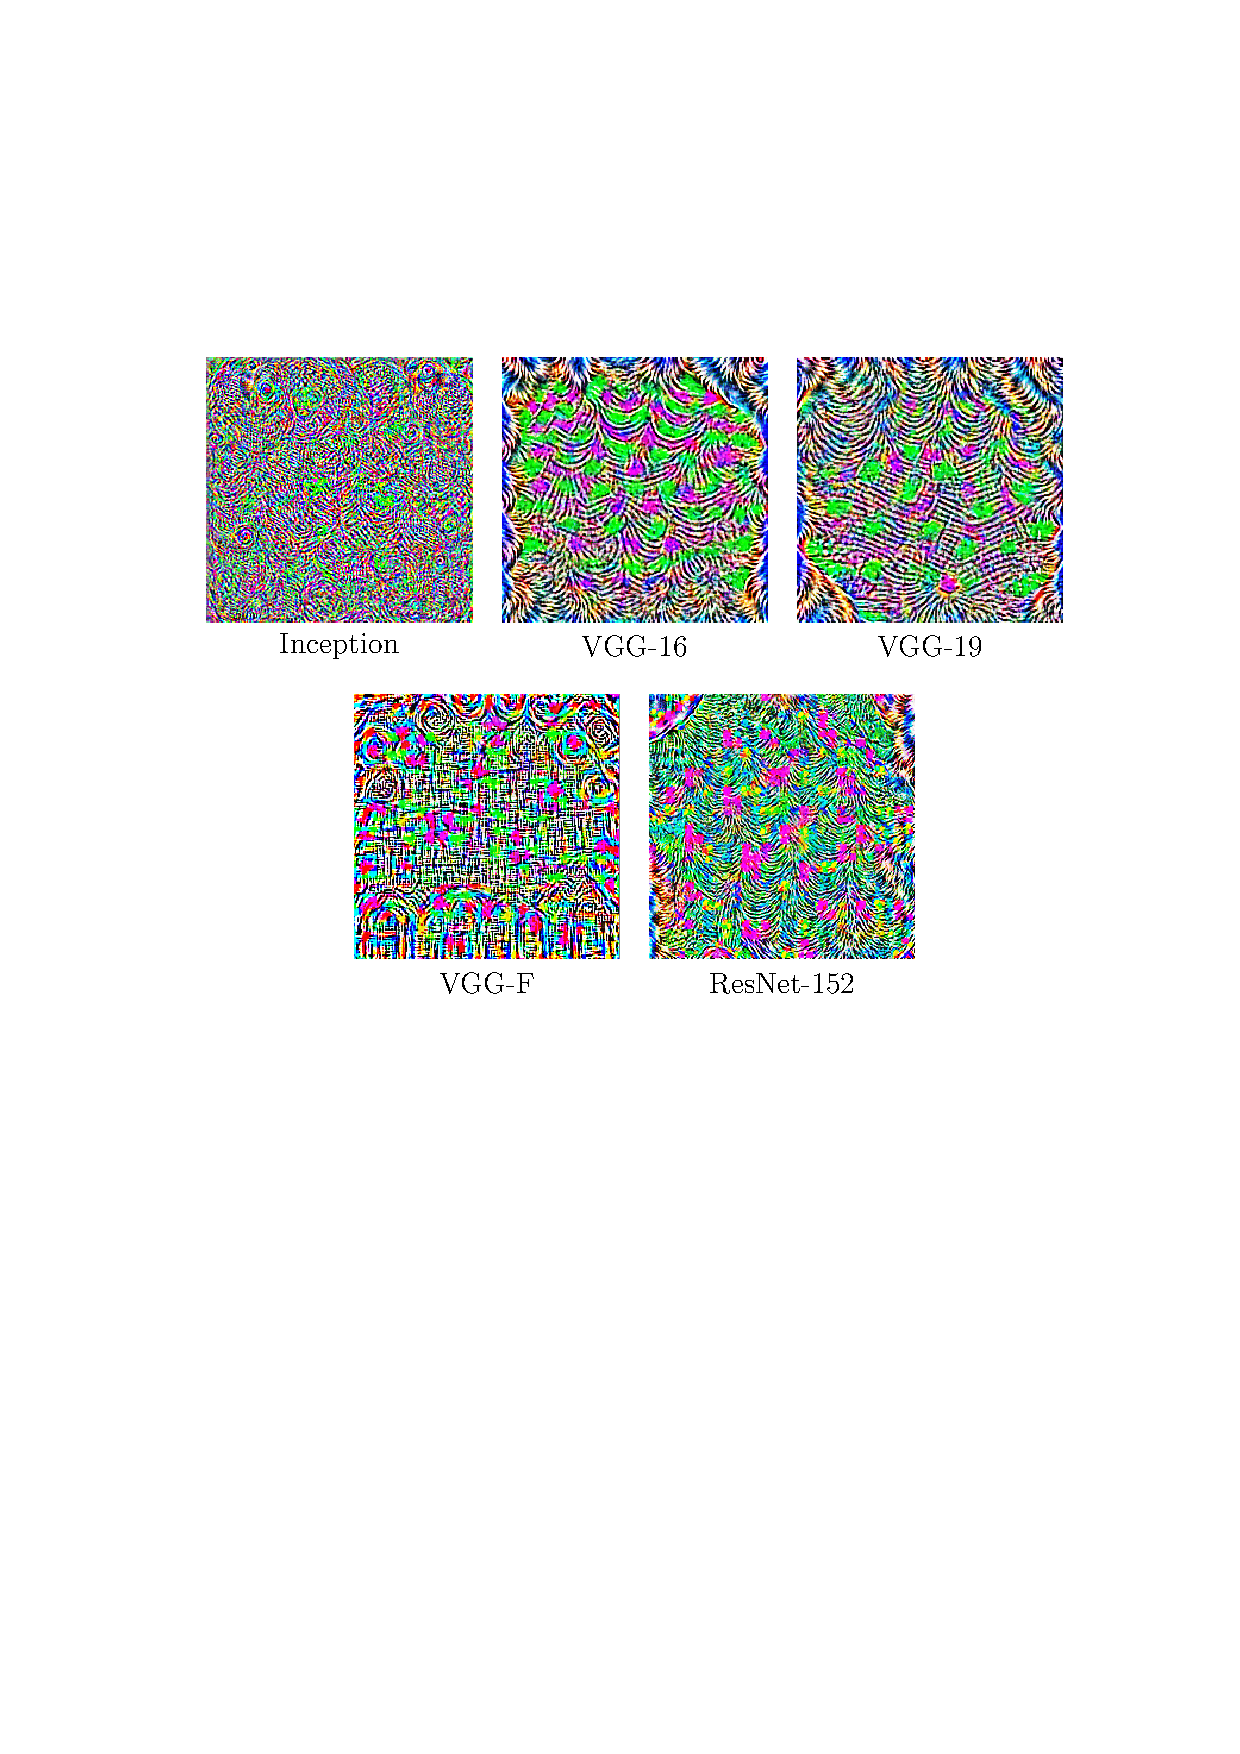
\includegraphics[clip, trim=3.8cm 12.8cm 2.8cm 5.8cm, width=1.0\textwidth]{plots_generierung/perturbationsFigure.pdf}
	\caption{Visualisation of the generated perturbations. To visualise the perturbations we shifted them by $+\xi$ and extended them to the entire colour space with a scalar multiplication.}\label{fig_stoerwerte}
\end{figure}

Fig.~\ref{fig_stoerwerte} shows the perturbations generated. In their general structure and appearance, they are similar to the ones reported in~\cite{moosavidezfooli_universal_2017}. In particular, the fine line-shaped structures in green and magenta are quite recognisable and are present also in the original results in~\cite{moosavidezfooli_universal_2017}. We believe that this indicates that deviations from the original results reported below stem from configuration details rather than a fundamental reproduction mistake. Therefore and despite the lower fooling rates reported below, we feel justified to use this setup to study our methods to generate a combined UAP for several networks. 

\bgroup

%\def\arraystretch{1.5}%  1 is the default, change whatever you need
\setlength\tabcolsep{0.2cm}
\begin{table}[htbp]
\centering
\caption{Fooling rates using the UAP method on the ImageNet validation set for several neural networks. Left values in bold are our reproduction results. The values to the right are the results reported in~\cite{moosavidezfooli_universal_2017}.}
\begin{tabular}{|c|c|c|c|c|c|c|c|c|c|c|c|}
\hline

			& \multicolumn{2}{|c|}{VGG-F}			&	\multicolumn{2}{|c|}{Inception}		&	\multicolumn{2}{|c|}{VGG-16}			&	\multicolumn{2}{|c|}{VGG-19}			&	\multicolumn{2}{|c|}{ResNet-152}	\\ \hline
VGG-F		& $\mathbf{90\%} $&$ 94\%$	&	$\mathbf{56\%} $&$ 48\%$	&	$\mathbf{32\%} $&$ 42\%$	&	$\mathbf{32\%} $&$ 42\%$	& 	$\mathbf{24\%} $&$ 47\%$		\\
Inception	& $\mathbf{42\%} $&$ 46\%$	&	$\mathbf{82\%} $&$ 79\%$	&	$\mathbf{16\%} $&$ 39\%$	&	$\mathbf{16\%} $&$ 40\%$	& 	$\mathbf{16\%} $&$ 46\%$	\\
VGG-16		& $\mathbf{46\%} $&$ 63\%$	&	$\mathbf{60\%} $&$ 57\%$	&	$\mathbf{59\%} $&$ 78\%$	&	$\mathbf{52\%} $&$ 73\%$	& 	$\mathbf{38\%} $&$ 63\%$	\\
VGG-19		& $\mathbf{45\%} $&$ 64\%$	&	$\mathbf{58\%} $&$ 54\%$	&	$\mathbf{51\%} $&$ 74\%$	&	$\mathbf{54\%} $&$ 78\%$	& 	$\mathbf{33\%} $&$ 58\%$	\\
ResNet-152	& $\mathbf{42\%} $&$ 46\%$	&	$\mathbf{55\%} $&$ 51\%$	&	$\mathbf{31\%} $&$ 47\%$	&	$\mathbf{33\%} $&$ 46\%$	& 	$\mathbf{73\%} $&$ 84\%$	\\
\hline 
\end{tabular}
\label{tbl_stoerraten_reprod_kreuz_linf}
\end{table}
\egroup

Tab.~\ref{tbl_stoerraten_reprod_kreuz_linf} shows the achieved fooling rates for the tested models (left values, in boldface) and the fooling rates reported by Moosavi-Dezfooli et al.~\cite{moosavidezfooli_universal_2017} (right values). The first column indicates the network used to generate the UAP while the first row gives the network on which the fooling rate is measured. The main diagonal therefore contains the self-fooling rates, i.e. the fooling rates achieved using the same model for generating the perturbation and measuring the fooling rate. 

To reproduce these numbers, several insufficiently documented design choices had to be researched. For example, the original results are not stated for a given epoch but using a stopping condition on the error rate. Values reported here are for epoch 20, at which point the mean value over the last 5 epochs typically varies by less than 0.005. Parameter values taken from and in the notation of~\cite{moosavi-dezfooli_deepfool_2016} are \(p=\infty\) and \(\xi=10\). We used a maximum of 10 DeepFool update iterations. The overshoot parameter \(\eta=0.02\) was again taken from~\cite{moosavi-dezfooli_deepfool_2016}. 

Another important parameter is the number of tested class boundaries, called \texttt{num\_classes}\footnote{As given in the code at https://github.com/LTS4/universal/}. It gives the number of class boundaries in whose direction a perturbation is searched for. Computation time is highly sensitive to this parameter, and checking all 1000 training boundaries of ImageNet was infeasible. Higher values generally improve the fooling performance, though exceptions are observed. 
Other minor parameters such as random initialisation values for the train-test split, etc. were taken from the provided code. We have tried to optimise these parameters using grid searches, but the available computing resources have limited these efforts. 

As part of this contribution we provide our code for the above reproduction effort and include the NEURIPS-2019 reproducibility checklist\footnote{See the file checklist.md in https://github.com/mauruskuehne/lwda-paper}.

\subsection{Evaluation of Approaches to Construct Universal Adversarial Perturbations for Multiple Neural Networks}\label{sec:EvaluationCombined}
In this section we present our results for constructing UAPs that make use of two neural networks. We discuss results for the two approaches presented in Sec.~\ref{sec:MultUAP}, the alternating generation of perturbations and the linear interpolation between UAP on individual networks.

The alternating generation of perturbations as given in Alg.~\ref{alg:1a} has been applied to the set of classifiers \(K=\left\{\text{Inception},\text{VGG-16}\right\}\). In Tab.~\ref{tab:vergleich_comb} the fooling rates are reported for these two networks and for ResNet-152. The table has two sections. In the upper section, the network listed in the first column is used to generate the perturbation. The columns give the fooling rates on the network given in the column title as well as their average as our measure for the generalisability of the UAPs. We include the original network in this average. 
The second section reports results by applying the alternating generation of UAPs and the interpolation method given in Eq.~(\ref{eq:interp}) using the value $\lambda=0.05$. 

Alg.~\ref{alg:1a} achieved results similar to the ones of a perturbation generated on VGG-16 only. Alg.~\ref{alg:1b} achieved slightly higher fooling rates on VGG-16 and ResNet-152 than a perturbation generated directly on VGG-16 (with an absolute increase of 2 and 3 percentage points, respectively). For Inception, the perturbation achieved a fooling rate of 67\%. This is 15\% below the measured self-fooling rate of Inception (82\%) but 7\% higher than the fooling rate achieved with a VGG-16 model. 

For a linear interpolation between the UAPs of VGG-16 and Inception V1, the best results were achieved for \(\lambda=0.05\) (see Eq.~(\ref{eq:interp})). Using this configuration, the fooling rates remained essentially unchanged compared to the UAP generated on VGG-16 only.
The small value \(\lambda=0.05\) results in a perturbation that is similar to the VGG-16 perturbation as the VGG-16 perturbation is weighted with \(1-\lambda=0.95\) while the Inception perturbation contributes only with a weight of 5\%. Choosing \(\lambda\in\left[0.1,0.15,\ldots,0.4\right]\) resulted in perturbations with lower fooling rates for both models with respect to the rates achieved by separately training UAPs on the two networks. For \(\lambda \in\left[0.4,1.0\right]\), the fooling rates for Inception improved again but did not exceed the fooling rate of a UAP generated on Inception itself. The fooling rate on VGG-16 continued to deteriorate, stabilising at a low fooling rate of \(\sim 15\%\) after \(\lambda\geq 0.65\). This suggests that linear interpolation does not result in improved fooling rates.
\begin{table}
\centering

\begin{tabular}{|c|c|c|c|c|c|}
\hline
											&	Inception	V1&	VGG-16		&	ResNet-152	& Average	\\ \hline
Inception V1 UAP							&	\(82\%\)		&	\(16\%\)	&	\(16\%\)	&38\%	\\
VGG-16 UAP								&	\(60\%\)		&	\(59\%\)	&	\(38\%\)	&52\%	\\
ResNet-152 UAP &	\(55\%\)		&	\(31\%\)	&	\(73\%\)&53\%		\\ \hline
linear interpolation with \(\lambda=0.05\)	&	\(60\%\)		&	\(59\%\)	&	\(38\%\)	&52\%\\
alternating generation of UAPs, Alg.~\ref{alg:1a}&	\(63\%\)		&	\(55\%\)	&	\(36\%\)	& \(51\%\)	\\
alternating generation of UAPs, Alg.~\ref{alg:1b}&	\(\mathbf{67}\%\)		&	\(\mathbf{61}\%\)	&	\(\mathbf{41}\%\)		&\(\mathbf{56}\)\%\\
\hline 
\end{tabular}

\caption{Comparison of the fooling rates by UAPs trained on individual networks (upper three rows) and of combination methods for several networks (lower three rows). Best values are shown in bold. Among the alternating generation variants (Alg.~\ref{alg:1a} and Alg.~\ref{alg:1b}) and the linear interpolation procedure (Eq.~(\ref{eq:interp})), Alg.~\ref{alg:1b} performs best with respect to the average fooling rate over all three networks. Results are reported on the validation set, using the $l_\infty$-norm, $\xi=10$ and 20 UAP iterations.}\label{tab:vergleich_comb}
\end{table}


\section{Discussion}\label{sec:Discussion}
\subsection{Reproduction of the Original Results on Universal Adversarial Perturbations}
For most models the fooling rates reported in the original paper could not be achieved, indicating that our reproduction results fell short of being satisfactory. For VGG-F, VGG-16, VGG-19 and ResNet-152 our self-fooling rates were between 4 and 24 absolute percentage points lower. For Inception we achieved a self-fooling rate 3 absolute percentage points higher than the one reported in the original paper. Further research is needed to state the precise conditions under which a reliable reproduction of the reported fooling rates is possible. As a step in this direction we have provided our code.

The non-diagonal values in Tab.~\ref{tbl_stoerraten_reprod_kreuz_linf} are large but typically significantly smaller than the diagonal values. They show a degree of transferability of UAPs generated with DeepFool to other models. Therefore, despite the reproducibility problems, these results broadly confirm that UAPs generated with DeepFool generalise to other network architectures. Nevertheless, it is clear that some aspects of UAPs are specific to a given neural network architecture. We discuss our results on finding a way to improve the non-diagonal elements (potentially at the cost of the diagonal ones) in the next section.
Interestingly, we achieved lower fooling rates than Moosavi-Dezfooli et al., except for the Inception network, for which we achieve 3 to 8 absolute percentage points higher fooling rates. This difference may be due to different stopping criteria, resulting in Moosavi-Dezfooli et al. running less optimisation epochs.
 Another possibility is that the chosen hyperparameter values for DeepFool and UAP might be particularly well suited or optimised for the Inception model. This in turn would explain the lower fooling rates achieved on other models.

\subsection{Alternating Generation of Perturbations and Linear Interpolation Be\-tween UAPs on Individual Networks}
As the results in Sec.~\ref{sec:EvaluationCombined} clearly show a linear interpolation between two UAPs does not give good results. This suggests that using a weighted average to combine UAPs is not a suitable approach to produce good UAPs for several neural networks. A more sophisticated UAP-combination procedure is clearly necessary to generate perturbations that fool both networks to a high degree.

The results given by the alternating generation of perturbations (Alg.~\ref{alg:1b}) are much better (see Tab.~\ref{tab:vergleich_comb}). The fooling rate of the perturbation generated jointly on Inception and VGG-16 is better than the ones generated on any one of the 
two networks. A perturbation generated on Inception achieves a fooling rate of 16\% on VGG-16 while a perturbation generated on VGG-16 achieves a fooling rate of 60\% on Inception. Both rates are lower than the ones of a perturbation generated jointly on Inception and VGG-16, achieving 67\% on Inception and 61\% on VGG-16. Furthermore, the fooling rate of a jointly trained UAP on Inception and VGG-16 on a third network (Resnet-152) is better than the fooling rate of both single-network UAPs. The UAP generated jointly on both networks even worked slightly better for VGG-16 than the one trained on VGG-16 alone. The reason for this effect and its statistical significance are not yet established. 

In judging these results, we note that estimates of their uncertainties are still lacking due to constraints on our computational resources. Ideally, one would like to provide mean and standard deviation values of all these numbers over multiple train-test splits as encouraged by the NEURIPS-2019 reproducibility checklist. Furthermore, the choice of the ImageNet training and testing data and the hyperparameter values (such as $p$, $\xi$, \texttt{num\_classes}, etc.) should be investigated. 

\section{Conclusions}\label{sec:conclusion}
The results reported here on generalising UAPs across several networks clearly have to be interpreted cautiously given the fact that even the reproduction of previously reported results has not been satisfactory. Establishing reproducibility standards for machine learning publications remains a crucial challenge that is hampering progress.

With the above caution in mind, the results reported here suggest that finding universal adversarial perturbations that generalise across different convolutional neural networks is not a hopeless endeavour. As we found, such a UAP is likely not a linear combination of UAPs of different networks but must be constructed in a more subtle way. Our best approach, Alg.~\ref{alg:1b}, most certainly is not optimal. Nevertheless it already shows some promising results: The generalisability of the fooling rates to ResNet-152 is enhanced by combining the UAPs of two networks, with respect to the UAPs generated on either one of the Inception or VGG-16 network. This suggests that combining several or even many networks might produce UAPs that are efficient on a whole class of trained 
convolutional neural networks.

\bibliography{KuehneToedtli}

\end{document}
